%%%%%%%%%%%%%%%%%%%%%%%%%%%%%%%%%%%%%%%%%%%%%%%%%%%%%%%%%%%%%%%%%%%%%%%%%%%%%%%%
\chapter{Proof of Concept Evaluation}\label{ch:validation}
%%%%%%%%%%%%%%%%%%%%%%%%%%%%%%%%%%%%%%%%%%%%%%%%%%%%%%%%%%%%%%%%%%%%%%%%%%%%%%%%


%%%%%%%%%%%%%%%%%%%%%%%%%%%%%%%%%%%%%%%%%%%%%%%%%%%%%%%%%%%%%%%%%%%%%%%%%%%%%%%%'
\section{Testbed and Validation}


As the experimental platform for validation we use Mininet-based emulated scenarios.  For reproducibility purposes, Table~\ref{tab:specifications} presents all relevant experimental details. All the required scripts are available on the SIMITAR code repository\cite{projeto-github}. We use SIMITAR v0.4.2 (Eulemur rubriventer)\footnote{ We label the tags of SIMITAR control version on GitHub as lemurs species names (\href{https://en.wikipedia.org/wiki/List_of_lemur_species}{https://en.wikipedia.org/wiki/List\_of\_lemur\_species})}, as tagged at the GitHub repository. We explore a tree topology (Fig. ~\ref{fig:topo-tree}), and a one-hop connection (Fig.~\ref{fig:topo-simple}). Both scenarios as  SDN networks with an OpenDayLight (Beryllium) controller. We use two pcap files. The first is a Skype capture (\textit{skype-pcap}), and the second (\textit{lgw10s-pcap}) corresponds to the first ten seconds of a gateway capture\footnote{\textit{skype-pcap}: available at \url{https://wiki.wireshark.org/SampleCaptures}, named \textit{SkypeIRC.cap}; lgw10s-pcap avaiable at \url{http://tcpreplay.appneta.com/wiki/captures.html} named \textit{bigFlows.pcap}}. Host host \textit{h1} (IPv4 address 10.0.0.1) has generated the traffic, and was captured by TCPDump\footnote{TCPDump is a tool for monitoring and capturing network packets\cite{web-tcpdump}.} on \textit{pcap} format. 

To compare the degree of realism of the generated traffic, we use the flows' cumulative distribution function (CDF)\cite{harpoon-validation}, and the Wavelet multi-resolution analysis\cite{swing-paper}. On both analysis, the closer the plots are, the more realistic is the traffic generated by SIMITAR. The flow’s cumulative distribution measures the ingress of new flows over time, and it is a measure similarity and evolution of the traffic at the flow-level. On the other hand, the wavelet multi-resolution analysis can extract traffic scaling characteristics and is a measure of similarity at the packet-level. If the curve decreases, this indicates a periodicity on that time scale exists. If the curve remains approximately constant, it indicates similarity to white-noise. Finally, if the traffic has self-similar characteristics around a particular time scale, its curve increases linearly. Table~\ref{tab:results-summary} presents a compendium of metrics extracted from the traffic, including the Hurst exponent, which is a metric of the traffic fractal level. Self-similar  processes, such as the network traffic, have its value between 0.5  and 1.0 ($0.5 < H < 1.0 $)\cite{selfsimilar-ethernet}.


\begin{table}[!ht]
    \centering
    \caption{Experiments specification table}
    \label{tab:specifications}
    \begin{tabular}{ll}
        \hline
        Processor            & Intel(R) Core(TM) i7-4770, 8 cores, CPU @ 3.40GHz \\
        RAM                  & 15.5 GB                                           \\
        HD                   & 1000 GB                                           \\
        Linux         & 4.8.0-59-generic                                  \\
        Ubuntu        & Ubuntu 16.10 (yakkety)                            \\
        SIMITAR       & v0.4.2 (Eulemur rubriventer)                      \\
        Mininet       & 2.3.0d1                                           \\
        Iperf         & iperf version 2.0.9 (1 June 2016) pthreads        \\
        Libtins       & 3.4-2                                             \\
        OpenDayLight  & 0.4.0-Beryllium                                   \\
        Octave        & 4.0.3                                             \\
        Pyshark       & 0.3.6.2                                     \\
        Wireshark     & 2.2.6+g32dac6a-2ubuntu0.16.10               \\
        Tcudump       & 4.9.0 \\
        libpcap       & 1.7.4\\
        \hline
    \end{tabular}
\end{table}

\begin{figure}[!thb]
    \centering
    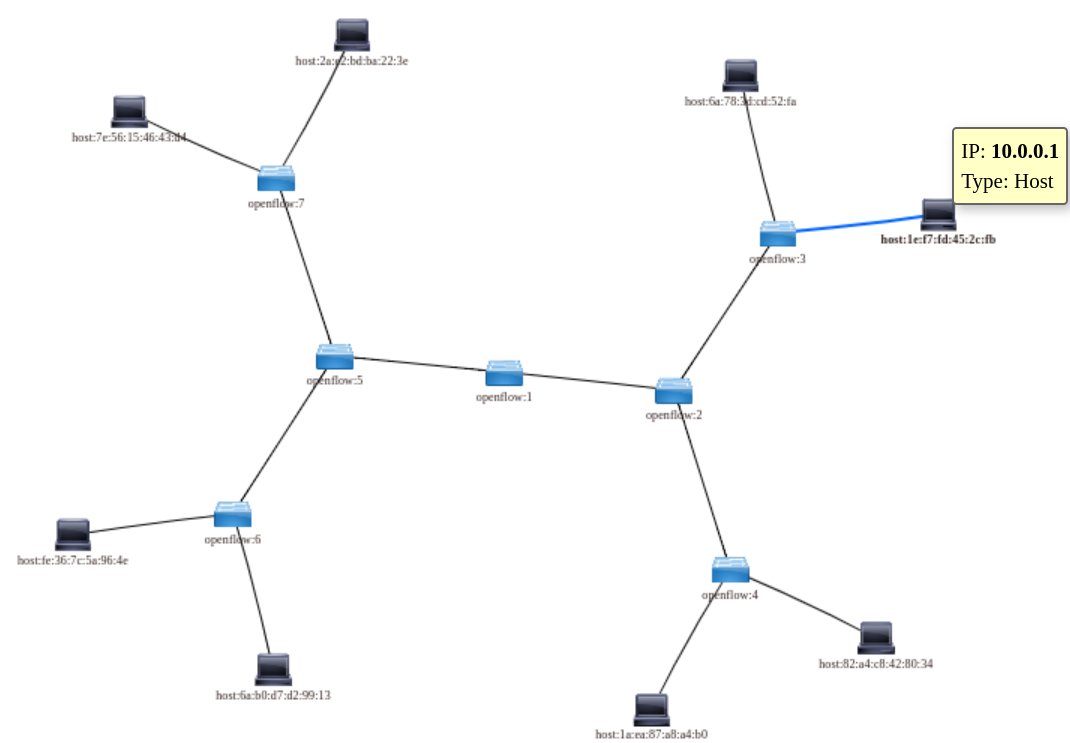
\includegraphics[width=\textwidth]{figures/ch5/topo-tree}
    \caption{Tree SDN topology emulated by mininet, and controlled by OpenDayLight Beryllium}
    \label{fig:topo-tree}
\end{figure}

\begin{figure}[!ht]
    \centering
    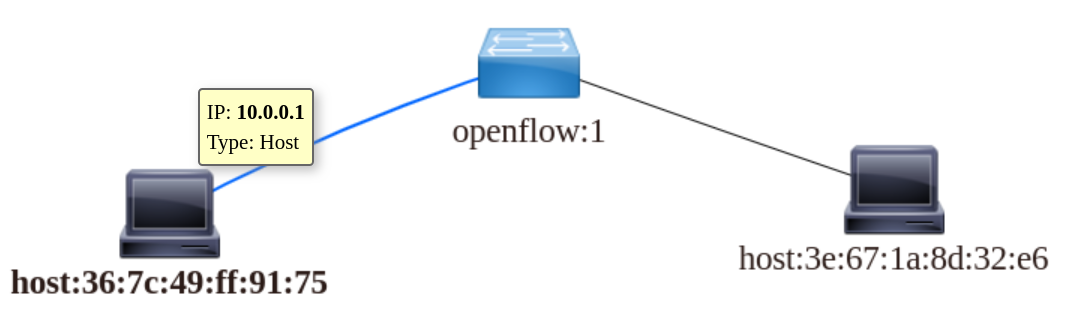
\includegraphics[width=0.8\textwidth]{figures/ch5/topo-simple}
    \caption{Single hop SDN topology emulated by mininet, and controlled by OpenDayLight Beryllium}
    \label{fig:topo-simple}
\end{figure}


\begin{table}[!htb]
	\centering
	\caption{Performed validations}
		\begin{tabular}{c c}
			\toprule
			\textbf{Metric Type} & \textbf{Validations} \\
			\midrule
			\makecell{Packet Based \\Metrics}                & \makecell{Data bit rate (kbps), Average packet\\
				rate (packets/s), Average packet size\\
				(bytes), Number of packets, Number of\\
				packets, Bandwidth over time}\\
			
			\makecell{Flow Based \\ Metrics}                & \makecell{Number of flows, Flows per second, \\
				Flows CDF distributions}\\
			
			\makecell{Fractal and Scaling \\ Characteristics} & \makecell{Hurst Exponent, Wavelet \\
				Multiresolution Analisis}\\
			\bottomrule
		\end{tabular}
	\label{tab:validation-tests-performed}
\end{table}


%%%%%%%%%%%%%%%%%%%%%%%%%%%%%%%%%%%%%%%%%%%%%%%%%%%%%%%%%%%%%%%%%%%%%%%%%%%%%%%%
\section{Results}


Figures ~\ref{fig:flows-cdf},~\ref{fig:wavelet} and Table~\ref{tab:results-summary} show the obtained results when comparing the original and the synthetic traffic generated by SIMITAR. We also illustrate the bandwidth traffic for one of the use cases in figure~\ref{fig:flows-bandwidth}. As we can see the generated traffics are not identical regarding bandwidth. However, both present similar fractal-like shape. The Hurst exponent of inter-packet times in every case has an error smaller than 10\% compared to the original in every case, i.e., the fractal-level of each synthetic traffic is indeed similar to the original trace.

The plot of flows per second seems much more accurate (Fig.~\ref{fig:flows-ps}), since most of the peaks match. Indeed, no visual lag between the plots. Even though the generated traffic is not identical to the original, the cumulative flow distribution obtained for every study-case is almost identical on every plot (Fig.~\ref{fig:flows-cdf}). The small differences on the curves result from threads and process concurrence for resources, in addition to noise from the sleep/wake processes on the thread signals. Since the operating system made the packet capture and timing, the packet capture buffer queue may have contributed as well. This result was our most significant achievement in our implementation. This result shows that our method of flow scheduling and independent traffic generation was effective and efficient in replicating the original traffic at the flow-level. However, the actual number of flows was more significant when SIMITAR used Iperf as the traffic generator API and slightly smaller when using libtins. This discrepancy can be explained because Iperf establishes additional connections to control the signaling and traffic statistics for every connection. On the other hand, with libtins, the number of flows is small, since a flow generation is aborted if the NetworkFlow flow class fails to create a new traffic flow. 

The results from the Wavelet multi-resolution analysis of inter-packet times vary in each case. The time resolution chosen was ten milliseconds, and it is represented in log 2 scale. The equation can calculate the time of each time-scale j: 

\begin{equation}
t = \frac{2^{j}}{100} [s]
\end{equation}

In the first case (Fig.~\ref{fig:iperfCdf}), SIMITAR reproduced Skype traffic, using Iperf in a single-hop scenario. On small time scales, both curves increased linearly, which indicates a fractal shape. However, at this point, they exhibit different slopes with the synthetic traces behaving closer to a white-noise shape. After the time scales 5 and 6 (300-600 milliseconds) scale, the error between the curves becomes almost negligible. We also observe a periodicity pattern at the time-scale of 9 seconds. Vishwanath and Vahdat\cite{swing-paper}  measured the same periodicity pattern; which appears to be an intrinsic characteristic of  TCP traffic. We observe some periodicity at 11 and 13 time-scales (20 and 80 seconds). 

In the second case (Fig.~\ref{fig:iperftreeCdf}), on a tree topology on small time scales, we identify behavior closer to white-noise on small scales, and similar results, but with more substantial energy levels on greater time scales. The diversity introduced by the topology and the concurrent signaling traffic caused by the other hosts and switches does explain the observed behavior since node signaling tends to be more randomized than user-generated traffic. Indeed, as we can see in Table~\ref{tab:specifications}, there are two hundred more packets captured on the client interface in the tree topology compared to the one-hop scenario. 

In the last two plots (Figures~\ref{fig:tinsCdf} and ~\ref{fig:tinsLgwCdf}), where we use libtins as the packet crafter, the energy level is higher, and the curves are less correlated. SIMITAR, in the current implementation, is not modeling inter-packet with libtins and sends packets as fast as possible, which explains this discrepancy. However, in the last scenario, due to the higher average throughput, the observed performance was better.


\begin{table}[!htb]
    \centering
    \caption{Sumary of results comparing the original traces (italic) and te traffic generated by SIMITAR, with the description of the scenario.}
    \label{tab:results-summary}
    \scalebox{0.87}{
\begin{tabular}{lcccccc}
    \hline
    \multicolumn{1}{c}{\multirow{3}{*}{}} & \multirow{3}{*}{\textit{skype-pcap}} & \multicolumn{1}{c}{\multirow{3}{*}{\begin{tabular}[c]{@{}c@{}}skype, \\ one-hop, \\ iperf\end{tabular}}} & \multicolumn{1}{c}{\multirow{3}{*}{\begin{tabular}[c]{@{}c@{}}skype, \\ tree, \\ iperf\end{tabular}}} & \multicolumn{1}{c}{\multirow{3}{*}{\begin{tabular}[c]{@{}c@{}}skype, \\ one-hop, \\ libtins\end{tabular}}} & \multirow{3}{*}{\textit{lgw10s-pcap}} & \multicolumn{1}{c}{\multirow{3}{*}{\begin{tabular}[c]{@{}c@{}}lgw10s, \\ one-hop, \\ libtins\end{tabular}}} \\
    \multicolumn{1}{c}{}                  &                             & \multicolumn{1}{c}{}                                                                                     & \multicolumn{1}{c}{}                                                                                  & \multicolumn{1}{c}{}                                                                                       &                              & \multicolumn{1}{c}{}                                                                                        \\
    \multicolumn{1}{c}{}                  &                             & \multicolumn{1}{c}{}                                                                                     & \multicolumn{1}{c}{}                                                                                  & \multicolumn{1}{c}{}                                                                                       &                              & \multicolumn{1}{c}{}                                                                                        \\ \hline
    Hurst Exponent                        & 0.601                       & 0.618                                                                                                    & 0.598                                                                                                 & 0.691                                                                                                      & 0.723                        & 0.738                                                                                                       \\
    Data bit rate (kbps)                  & 7                           & 19                                                                                                       & 19                                                                                                    & 12                                                                                                         & 7252                         & 6790                                                                                                        \\
    Average packet rate (packets/s)       & 3                           & 4                                                                                                        & 5                                                                                                     & 6                                                                                                          & 2483                         & 2440                                                                                                        \\
    Average packet size (bytes)           & 260,89                      & 549,05                                                                                                   & 481,14                                                                                                & 224,68                                                                                                     & 365,00                       & 347,85                                                                                                      \\
    Number of packets                     & 1071                        & 1428                                                                                                     & 1604                                                                                                  & 2127                                                                                                       & 24 k                         & 24 k                                                                                                        \\
    Number of flows                       & 167                         & 350                                                                                                      & 325                                                                                                   & 162                                                                                                        & 3350                         & 3264                                                                                                        \\ \hline
\end{tabular}
    }
\end{table}


\begin{figure}[ph]
% Bandwidth
\begin{figure}[H]
    \centering
    \subfloat[\textit{Iperf, single-hop, skype-pcap}]{
        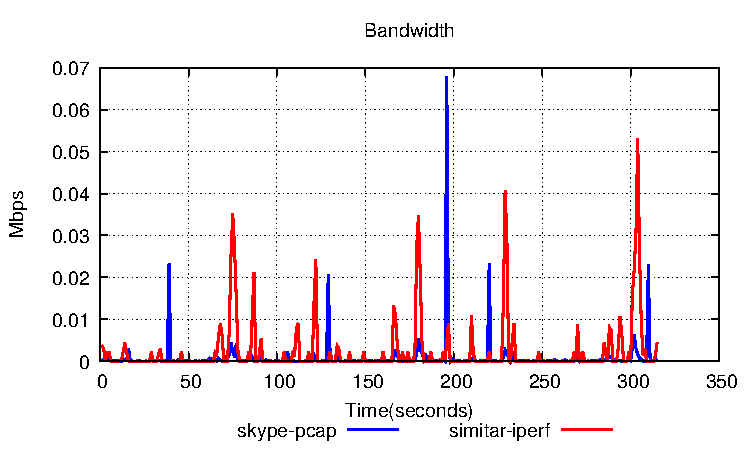
\includegraphics[width=72mm]{figures/ch5/skype-iperf-Bandwidth.pdf}
        \label{fig:iperfBw}
    }
    \hspace{0mm}
    \subfloat[\textit{Iperf, tree, skype-pcap}]{
        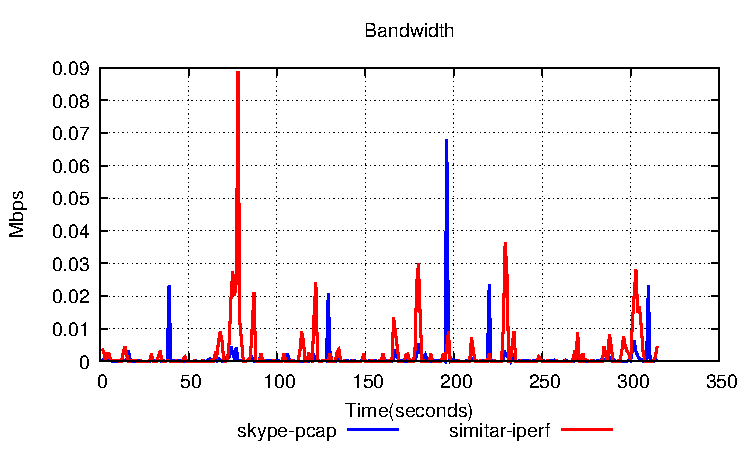
\includegraphics[width=72mm]{figures/ch5/skype-tree-iperf-Bandwidth.pdf}
        \label{fig:iperftreeBw}
    }
    \hspace{0mm}
    \subfloat[\textit{libtins, single-hop, skype-pcap}]{
        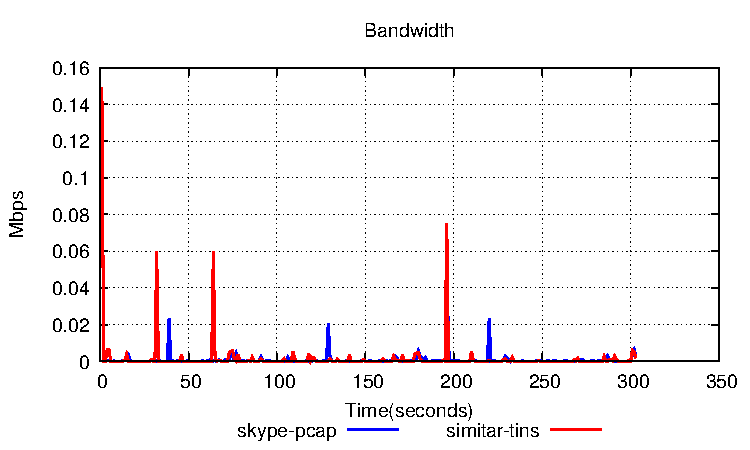
\includegraphics[width=72mm]{figures/ch5/skype-tins-Bandwidth.pdf}
        \label{fig:tinsBw}
    }
    \hspace{0mm}
    \subfloat[\textit{libtins, single-hop, langw10s-pcap}]{
        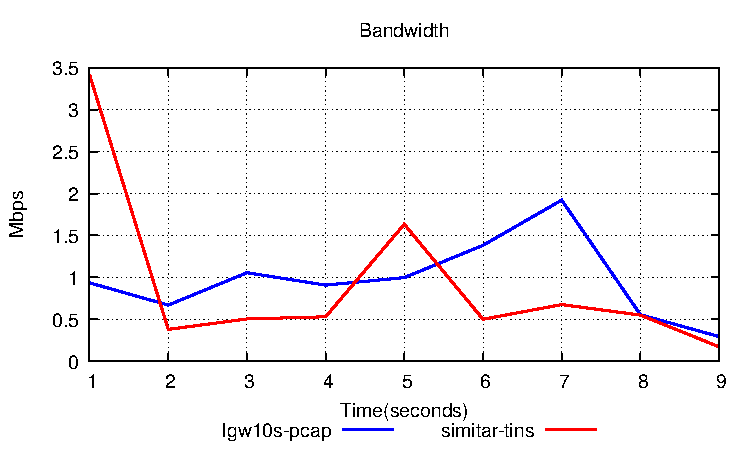
\includegraphics[width=72mm]{figures/ch5/lgw-tins-Bandwidth.pdf}
        \label{fig:tinsLgwBw}
    }
    \hspace{0mm}
    \caption{Traces bandwidth.}
    \label{fig:flows-bandwidth}
\end{figure}
% Flows per second
\begin{figure}[H]
    \centering
    \subfloat[\textit{Iperf, single-hop, skype-pcap}]{
        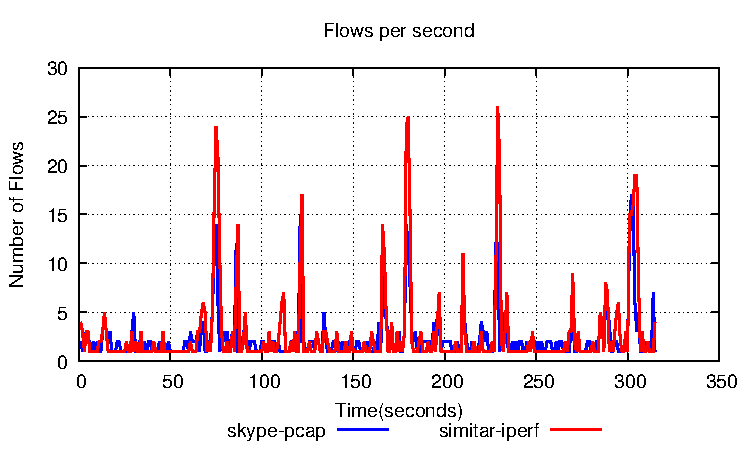
\includegraphics[width=72mm]{figures/ch5/skype-iperf-FlowsPs.pdf}
        \label{fig:iperfFps}
    }
    \hspace{0mm}
    \subfloat[\textit{Iperf, tree, skype-pcap}]{
        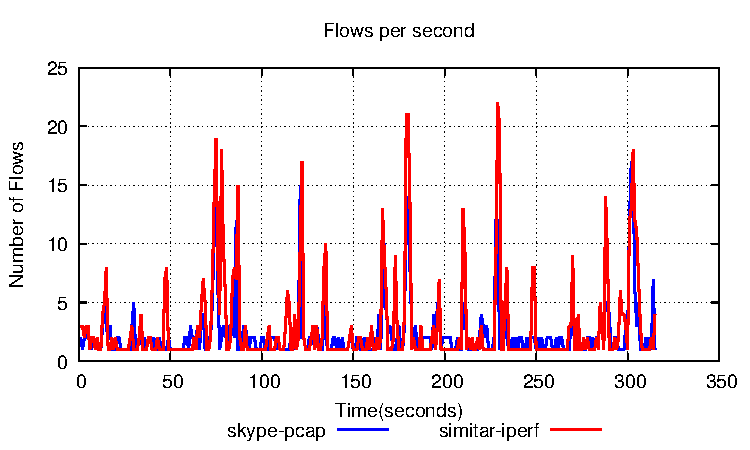
\includegraphics[width=72mm]{figures/ch5/skype-tree-iperf-FlowsPs.pdf}
        \label{fig:iperftreeFps}
    }
    \hspace{0mm}
    \subfloat[\textit{libtins, single-hop, skype-pcap}]{
        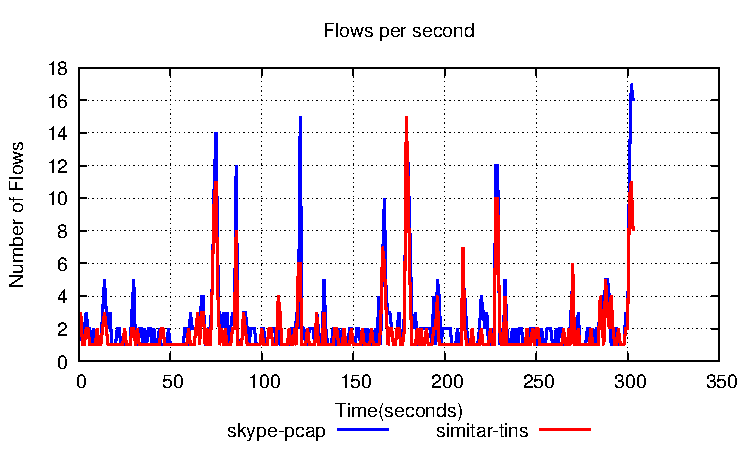
\includegraphics[width=72mm]{figures/ch5/skype-tins-FlowsPs.pdf}
        \label{fig:tinsFps}
    }
    \hspace{0mm}
    \subfloat[\textit{libtins, single-hop, langw10s-pcap}]{
        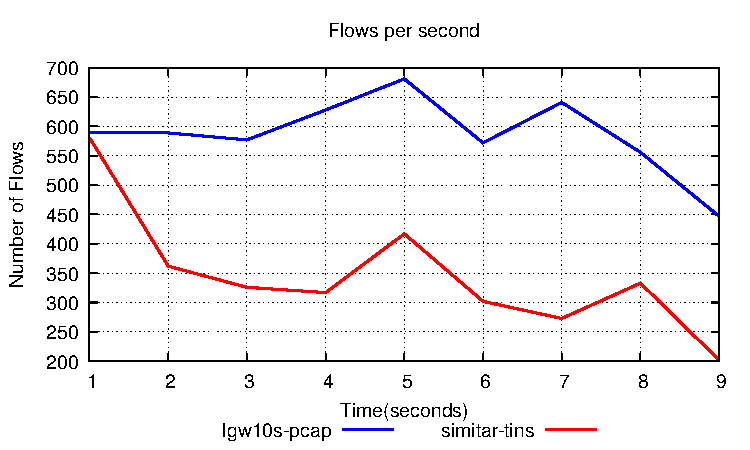
\includegraphics[width=72mm]{figures/ch5/lgw-tins-FlowsPs.pdf}
        \label{fig:tinsLgwFps}
    }
    \hspace{0mm}
    \caption{Flow per seconds}
    \label{fig:flows-ps}
\end{figure}
\end{figure}
\clearpage

\begin{figure}[ph]
% Flow CDF
\begin{figure}[H]
    \centering
    \subfloat[\textit{Iperf, single-hop, skype-pcap}]{
        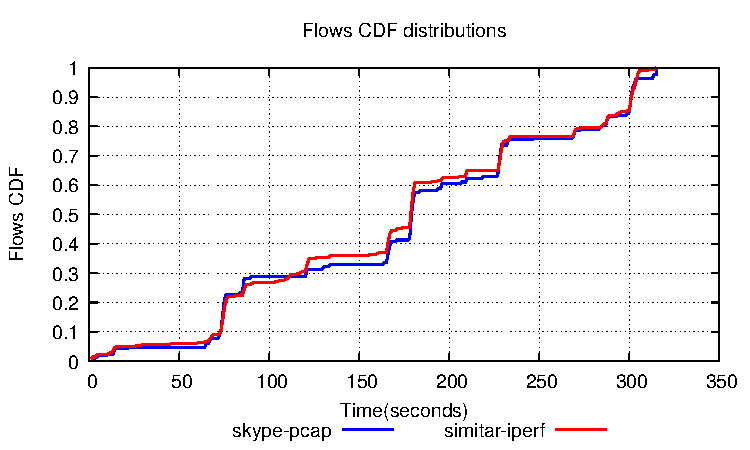
\includegraphics[width=72mm]{figures/ch5/skype-iperf-FlowCdf.pdf}
        \label{fig:iperfCdf}
    }
    \hspace{0mm}
    \subfloat[\textit{Iperf, tree, skype-pcap}]{
        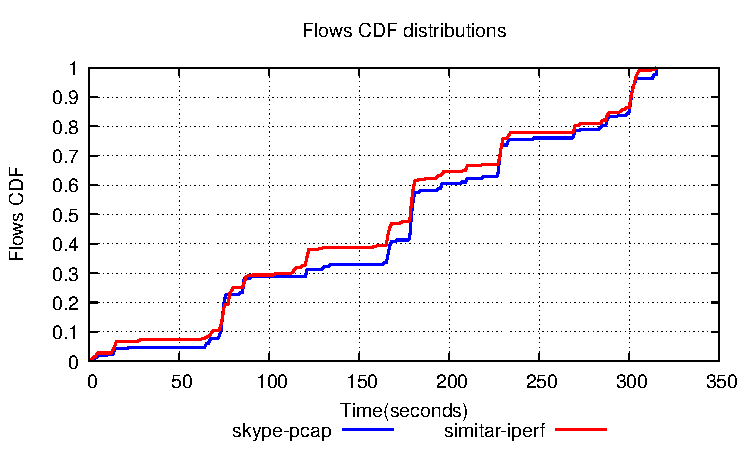
\includegraphics[width=72mm]{figures/ch5/skype-tree-iperf-FlowCdf.pdf}
        \label{fig:iperftreeCdf}
    }
    \hspace{0mm}
    \subfloat[\textit{libtins, single-hop, skype-pcap}]{
        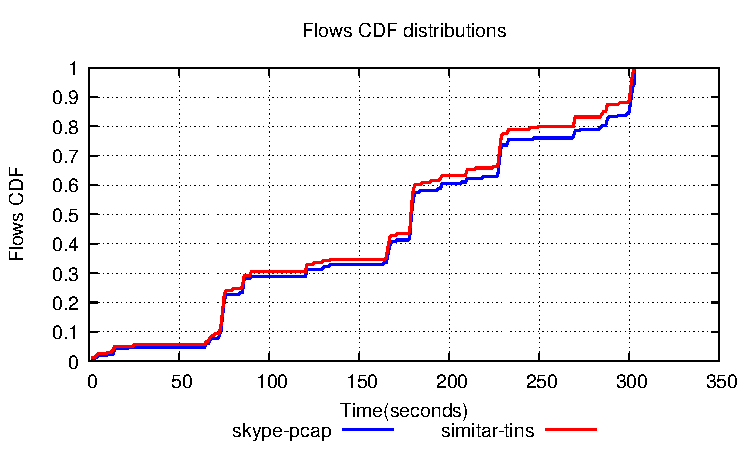
\includegraphics[width=72mm]{figures/ch5/skype-tins-FlowCdf.pdf}
        \label{fig:tinsCdf}
    }
    \hspace{0mm}
    \subfloat[\textit{libtins, single-hop, langw10s-pcap}]{
        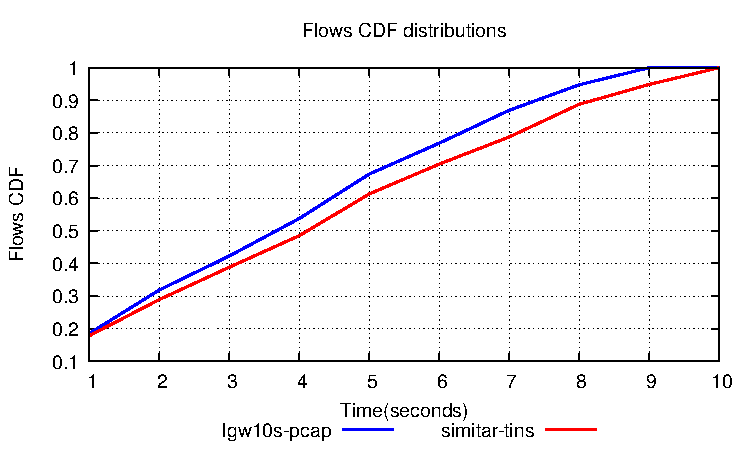
\includegraphics[width=72mm]{figures/ch5/lgw-tins-FlowCdf.pdf}
        \label{fig:tinsLgwCdf}
    }
    \hspace{0mm}
    \caption{Flows cumulative distributions.}
    \label{fig:flows-cdf}
\end{figure}
% Wavelet
\begin{figure}[H]
    \centering
    \subfloat[\textit{Iperf, single-hop, skype-pcap}]{
        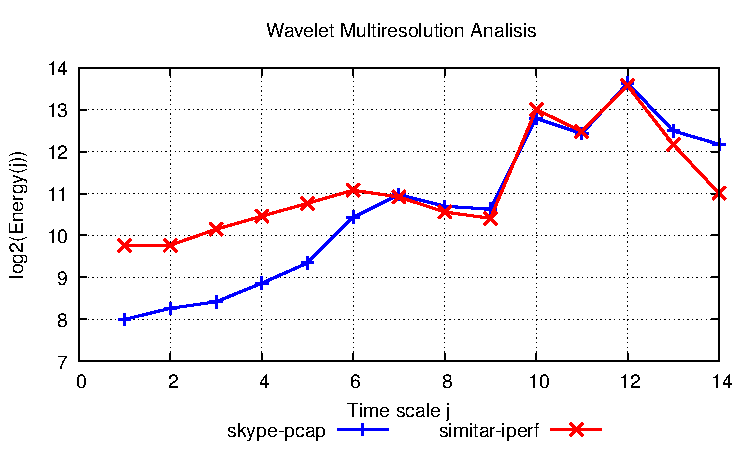
\includegraphics[width=72mm]{figures/ch5/skype-iperf-WaveletMREA.pdf}
        \label{fig:iperfWaveletMREA}
    }
    \hspace{0mm}
    \subfloat[\textit{Iperf, tree, skype-pcap}]{
        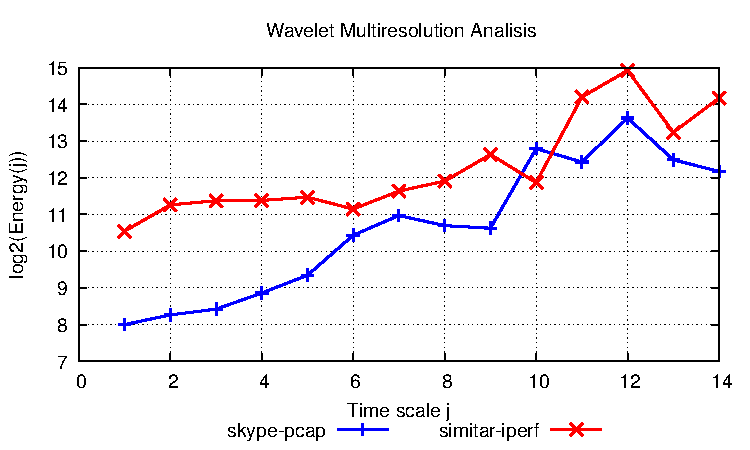
\includegraphics[width=72mm]{figures/ch5/skype-tree-iperf-WaveletMREA.pdf}
        \label{fig:iperftreeWaveletMREA}
    }
    \hspace{0mm}
    \subfloat[\textit{libtins, single-hop, skype-pcap}]{
        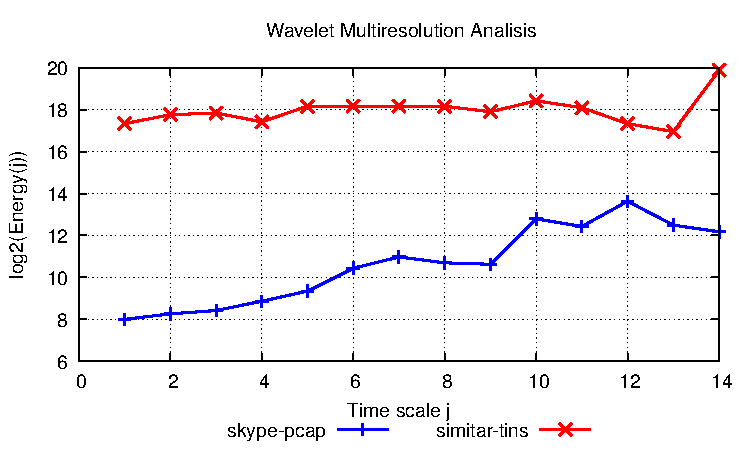
\includegraphics[width=72mm]{figures/ch5/skype-tins-WaveletMREA.pdf}
        \label{fig:tinsWaveletMREA}
    }
    \hspace{0mm}
        \subfloat[\textit{libtins, single-hop, langw10s-pcap}]{
            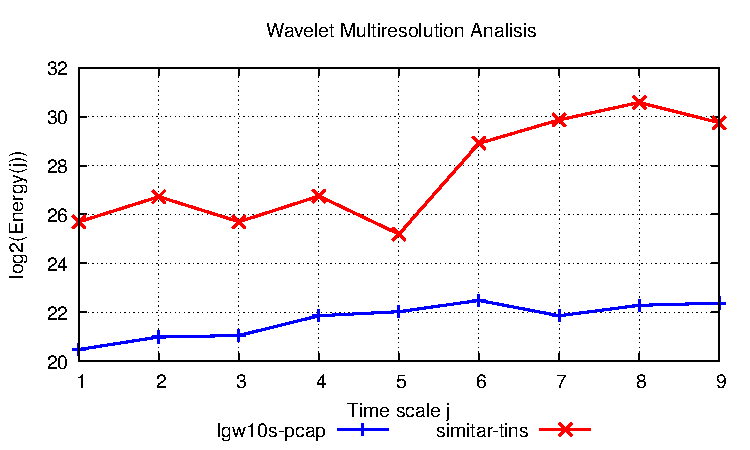
\includegraphics[width=72mm]{figures/ch5/lgw-tins-WaveletMREA.pdf}
            \label{fig:tinsLgwWaveletMREA}
        }
        \hspace{0mm}
    \caption{Wavelet multiresolution energy analysis.}
    \label{fig:wavelet}
\end{figure}
\end{figure}
\clearpage


%%%%%%%%%%%%%%%%%%%%%%%%%%%%%%%%%%%%%%%%%%%%%%%%%%%%%%%%%%%%%%%%%%%%%%%%%%%%%%%%
\section{Conclusions}


We present SIMITAR as a tool and methodology to attend the evolving needs of rich and realistic network traffic experiments working at both flow-  and packet-level. At the flow-level, our methodology already achieves high fidelity results. The cumulative distribution of flows is almost identical in each case. From the perspective of benchmarking of a middle-boxes or SDN switches, this is a valuable result, since their performance, especially in SW implementations, largely depend on the number and characteristics of the stimuli flows. However, because of packets exchanged by background signaling connections, the traffic generated by Iperf, even following the same cumulative flow distribution, ended up creating more streams then expected.  

At the packet level, the current results with Iperf replicate with high accuracy the scaling characteristics of the first traffic, and the number of generated packets are not far than the expected.  Despite all identified optimization, the results are more than satisfactory and prove the potential of the proposed methodology. At the flow-level, our results are at least as good as those achieved by best-of-breed related work like Harpoon and Swing.  On the scaling characteristics, using lightweight traces, the results have been of comparable in quality.
